\section{Opis korišćenih tehnologija i alata}

Programsko rešenje je razvijeno uz pomoć \textit{Java} programskog jezika i  \textit{Eclipse} programskog razvojnog okruženja prvenstveno namenjenog za razvoj \textit{Java} aplikacija. Pored \textit{Jave} \textit{Eclipse} podržava i druge programske jezike \cite{Eclipse}. Izgled \textit{Eclipse} razvojnog okruženja je prikazan na slici \ref{img:eclipse}.

\begin{figure}[ht]
\begin{center}
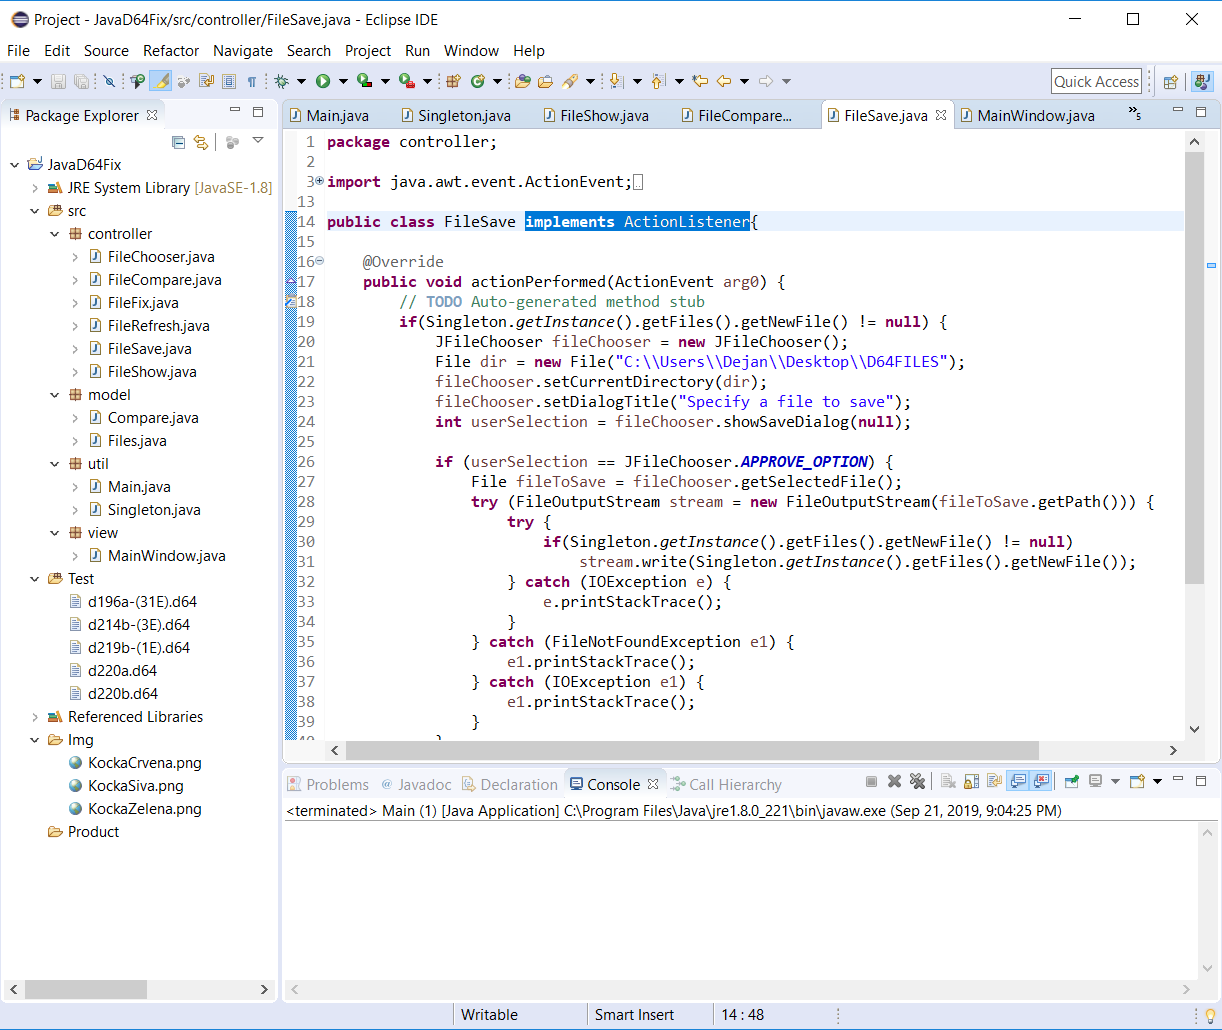
\includegraphics[width=\textwidth]{img/EclipseIDE.png}
\caption{Eclipse}
\label{img:eclipse}
\end{center}
\end{figure}

Za rad sa grafičkim elementima korišćen je \textit{Swing} radni okvir koji obezbedjuje skup grafičkih komponenti uz pomoć kojih realizujemo grafički korisnički interface u java programskom jeziku.